\documentclass{article}
\usepackage{amsmath}
\usepackage{graphicx}
\usepackage{stix}
\usepackage{listings}
\usepackage{xcolor}
\usepackage{caption}

\newcommand{\MuchLess}{\mathbin{\rotatebox[origin=c]{90}{$\Wedge$}}}
\newcommand{\xor}{\oplus}
\newcommand{\corr}[2]{\rho\left( #1 , #2 \right)}
\newcommand{\cov}[2]{\textit{cov}\left( #1 , #2 \right)}
\newcommand{\var}[1]{\textit{var}\left( #1 \right)}
\newcommand{\Exp}[1]{\textit{E}\left( #1 \right)}

\newcommand{\A}[1]{A_{t-#1}}
\renewcommand{\a}[1]{a_{t-#1}}
\newcommand{\B}[1]{B_{t-#1}}
\renewcommand{\b}[1]{b_{t-#1}}


\lstdefinestyle{mystyle}{
    % backgroundcolor=\color{backcolour},   
    commentstyle=\color{gray},
    keywordstyle=\color{magenta},
    numberstyle=\tiny\color{lightgray},
    % stringstyle=\color{codepurple},
    basicstyle=\ttfamily\footnotesize,
    % breakatwhitespace=false,         
    % breaklines=true,                 
    captionpos=b,                    
    keepspaces=true,                 
    numbers=left,                    
    numbersep=5pt,                  
    showspaces=false,                
    showstringspaces=false,
    showtabs=false,                  
    tabsize=2
}

\lstset{style=mystyle}



\title{Multiple Independent Streams of Random Numbers on FPGAs}
\author{Andrew W. Rose}

\begin{document}

\maketitle

\section{Introduction}

FPGAs are programmable-logic devices that provide bit-level parallelism and pipe-lining of computation. Modern FPGAs feature dedicated DSP and block-ram cores to reduce the consumption of logic-cells used for mathematical and memory application, but these resources are usually limited in number and in high demand, so are considered ``precious''. Since FPGAs operate at the bit-level, within the logic-cells bit-shuffling operations (including the traditional bit-shift and rotation operations) are available at no additional cost in terms of neither resources nor latency. For this reason, the Xoshiro and Xoroshiro PRNGs are an excellent fit for generating a stream of pseudo-random numbers in FPGAs, although the shuffling-stages proposed for these PRNGs, which are based on 64-bit addition and multiplication, should not necessarily be expected to be so well suited. 

A practical consideration when designing for FPGAs is that large ``fanouts'' of signals and long path-lengths invariably fail to meet the timing constraints at high clock-speeds or in congested designs, and so clocking outputs through word-wise shift-registers is a more favoured paradigm.

\section{Implementation of the Xoshiro256 PRNG in FPGAs}

All firmware discussed in this document has been implemented in VHDL-2008. All simulation was performed with Mentor/Siemens Modelsim. All synthesis and implementation was performed using the Xilinx Vivado 2020.2 toolkit, targetting a XCKU15P-2 Kintex Ultrascale+ FPGA, setting ``FlattenHierarchy'' to ``None'' and ``Strategy'' to ``AreaOptimized'', and default settings otherwise. Implementations were performed setting the nominal clock-speeds to 100MHz and 750MHz.

The Xoshiro256 algorithm was implemented in VHDL, requiring only two lines of functional code, listing \ref{lst:Xoshiro256}. The implementation produces a new random number on the output on every clock-cycle and can close timing on nominal clock-frequencies of 750MHz.

The plus-plus and star-star scramblers were compared, and shown to be functionally identical in an FPGA: Since $x*5 = (x*4) + x = (x << 2) + x = w + x$, and similarly for $x*9$, and since shift operations have no cost in an FPGA, the star-star scrambler, $\left( \left( x * 5 \right) <<< 7 \right) * 9$, is identical in computational complexity to the plus-plus scrambler, $\left( \left( x + y \right) <<< 7 \right) + y$. However, these operations need to be pipelined --- in this case across three steps for simplicity and clarity\footnote{Two steps could be used instead of three for lower latency and resources, but at a non-negligible cost to code readability} --- and in the plus-plus case, this also requires pipelining the final argument twice, increasing the register requirements, and so only the star-star scrambler was implemented in VHDL, requiring only a single line of functional code, listing \ref{lst:StarStar}. The implementation is fully pipelined, handling a new number on every clock-cycle, and can close timing on nominal clock-frequencies of 750MHz.

\begin{minipage}{1.0\textwidth}
\centering
\begin{lstlisting}[language=VHDL, caption={The Xoshiro256 PRNG implemented in VHDL. Although the functional code is shown spread over lines 10-16 here, the working code uses only two.} , label=lst:Xoshiro256]
ARCHITECTURE rtl OF Xoshiro256 IS
  -- s( -2 to -1 ) are not actually part of the state;
  --   Used for convenience.
  SIGNAL s : tArray( -2 TO 3 ) := ( Seed( 2 ) XOR Seed( 0 ) , 
                                    Seed( 3 ) XOR Seed( 1 ) , 
                                    Seed( 0 ) , Seed( 1 ) , 
                                    Seed( 2 ) , Seed( 3 ) );
BEGIN
  DataOut       <= s(1); -- Mapping
  s( -2 TO -1 ) <= ( s(2) XOR s(0)  , 
                     s(3) XOR s(1) ); -- Concurrent
  s(  0 TO  3 ) <= ( s(0) XOR s(-1) , 
                     s(1) XOR s(-2) , 
                     s(-2) XOR SHIFT_LEFT( s(1) , 17 ) , 
                     ROTATE_LEFT( s(-1) , 45 ) ) 
                   WHEN RISING_EDGE( Clk ); -- Clocked
END ARCHITECTURE rtl;
\end{lstlisting}
\end{minipage}

\begin{minipage}{1.0\textwidth}
\centering
\begin{lstlisting}[language=VHDL, caption={The star-star scrambler implemented in VHDL. Although the functional code is shown spread over lines 5-8 here, the working code uses only one.} , label=lst:StarStar]
ARCHITECTURE rtl OF StarStarScrambler IS
  SIGNAL Pipeline : tArray( 0 TO 2 ) := (OTHERS=>(OTHERS=>'0'));
BEGIN
  DataOut  <= Pipeline(2); -- Mapping
  Pipeline <= ( DataIn + SHIFT_LEFT( DataIn , 2 ) , 
                ROTATE_LEFT( Pipeline(0) , 7 ) , 
                Pipeline(1) + SHIFT_LEFT( Pipeline(1) , 3 ) ) 
              WHEN RISING_EDGE( Clk ); -- Clocked 
END ARCHITECTURE rtl;
\end{lstlisting}
\end{minipage}

\section{MISRN scheme 1}

Consider two generators producing two binary uniformly-distributed sequences, $A$ and $B$, the outputs of which are fed into a pair of word-wise shift registers. Let us consider orienting the shift registers in ``opposite directions'' and aligning the registers. Since the shift-registers are oppositely aligned, it is clear that the pairing of data at any node at any point in time is unique. We then consider that each node produces an unbiased output, $\alpha$, as a function of the two inputs: The simplest such function is the exclusive-or (XOR); we could also consider a shuffling of the bits (either random or systematic) in each input word, since these operations ``come for free'', but such a shuffling makes the process less amenable to verification, so we shall not consider this any further. We express this graphically in Figure \ref{fig:scheme1}, and mathematically as $\alpha^t_{(i,j)} = \A{i} \xor \B{j}$, where $t$ is the ``time'' in clock-cycles, and $(i,j)$ is an instance index indicating the ``distance'' from each generator. Noting that $i+j = N-1$, where $N$ is the number of cells in the shift-register, we could clearly replace the double index with a single index, but for clarity and symmetry, the double index is preferred.

\begin{figure}[ht]
\centering
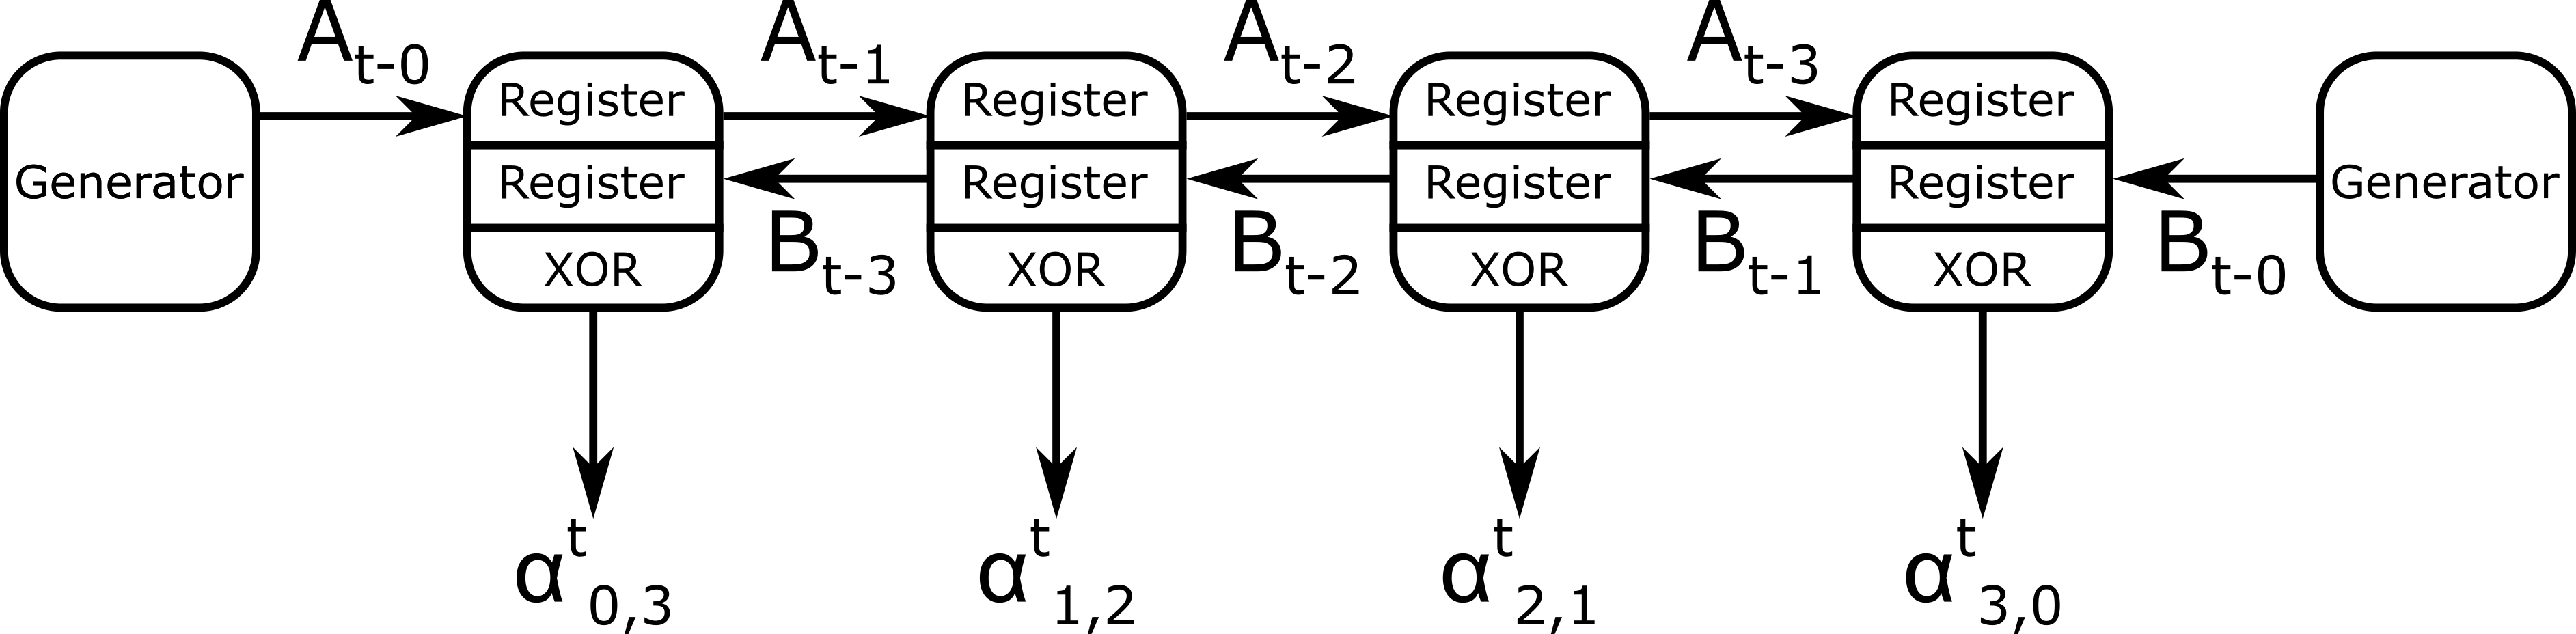
\includegraphics[width=\textwidth]{MISRN.png}
\caption{First scheme for producing MISRN via the exclusive-or of two streams with different timing offsets}
\label{fig:scheme1}
\end{figure}

\begin{minipage}{1.0\textwidth}
\centering
\begin{lstlisting}[language=VHDL, caption={Scheme 1 implemented in VHDL. Although the functional code is shown spread over lines 5-10 here, the working code uses only three.} , label=lst:Scheme1]
ARCHITECTURE rtl OF XorChain1 IS
  SIGNAL PipelineA : tArray( 0 to N-1 ) := OTHERS=>(OTHERS=>'0'));
  SIGNAL PipelineB : tArray( 0 to N-1 ) := OTHERS=>(OTHERS=>'0'));
BEGIN
  PipelineA <= ( DataInA & PipelineA( 0 to N-2 ) )
               WHEN RISING_EDGE( Clk ); -- Pipeline
  PipelineB <= ( PipelineB( 1 to N-1 ) & DataInB )
               WHEN RISING_EDGE( Clk ); -- Pipeline
  DataOut   <= ( PipelineA XOR PipelineB )
               WHEN RISING_EDGE( Clk ); -- XOR
END ARCHITECTURE rtl;
\end{lstlisting}
\end{minipage}

\subsection{Formalizing the independence}

Clearly, input $A$ to $\alpha_{i,j}$ at time $t$ is the same as input $A$ to $\alpha_{i+\Delta,j-\Delta}$ at time $t+\Delta$, and so if there is significant correlation between $B$ at times $t$ and $t-\Delta$, then there will also be significant correlation between $\alpha_{i,j}$ and $\alpha_{i+\Delta,j-\Delta}$. As long as any time-correlation in $B$ exceeds the length of the chain, then we should have no systematic correlations. Let us formalise this: To make XOR amenable to mathematical study, we consider the linear sequence transform $X \to x = 1 - 2X$ which respectively map the elements of $A$, $B$ from the range \{0,1\} to sequences $a$, $b$ in the range \{-1,1\}, so that the XOR operation may be replaced by multiplication, $A \xor B = a \cdot b$. 

The expectation value, variance and covariance of the transformed variables are, respectively,
\begin{align}
    \Exp{a} = & 1 - 2\Exp{A} \\
    \var{a} = & 4 \var{A} \\
  \cov{a}{b} = & 4 \cov{A}{B}
\end{align}

As $A$ is uniformly distributed, $\Exp{A} = \frac{1}{2}$ and $\var{A} = \frac{1}{4}$, so $\Exp{a} = 0$ and $\var{a} = 1$, and identically for $B$ and $b$.

The variance of the XOR function can then be defined as
\begin{align}
\var{A \xor B} = & \frac{1}{4} \var{a \cdot b} \\
                 = & \frac{1}{4} \left( \var{a} \cdot \var{b} + \var{a} \cdot \Exp{b}^2 + \Exp{a}^2 \cdot \var{b} \right) \\
                 = & \frac{1}{4} \left( 1 \cdot 1 + 1 \cdot 0 + 0 \cdot 1 \right) \\
                 = & \frac{1}{4} \label{eqn:var_xor}
\end{align}


Considering two outputs, $\alpha_{i,j}$ and $\alpha_{k,l}$. We may then define the correlation, $\rho$, between them as 
\begin{align}
  \corr{\alpha_{i,j}}{\alpha_{k,l}} = \frac{\cov{\alpha_{i,j}}{\alpha_{k,l}}}{\sqrt{\var{\alpha_{i,j}} \cdot \var{\alpha_{k,l}}}}
\end{align}
 
and, using the various results above,
\begin{align}
  \corr{\alpha_{i,j}}{\alpha_{k,l}} = & \frac{\cov{\A{i} \xor \B{j}}{\A{k} \xor \B{l}}}{\sqrt{\var{\A{i} \xor \B{j}} \cdot \var{\A{k} \xor \B{l}}}} \\
                                    = & \frac{\cov{\A{i} \xor \B{j}}{\A{k} \xor \B{l}}}{\sqrt{\frac{1}{4} \cdot \frac{1}{4}}} \\
                                    = & 4 \cov{\A{i} \xor \B{j}}{\A{k} \xor \B{l}} \\
                                    = & \cov{\a{i} \cdot \b{j}}{\a{k} \cdot \b{l}}
\end{align}

And by the definition of the covariance
\begin{align}
  \corr{\alpha_{i,j}}{\alpha_{k,l}} = & \Exp{\a{i} \cdot \b{j} \cdot \a{k} \cdot \b{l}} \nonumber \\
                                      & - \Exp{\a{i} \cdot \b{j}} \cdot \Exp{\a{k} \cdot \b{l}}
\end{align}

Assuming that $A$ and $B$ are independent, 
\begin{align}
  \Exp{\a{i} \cdot \b{j}} = & \Exp{\a{i}} \cdot \Exp{\b{j}} \\
                          = & 0 \cdot 0 \\
                          = & 0
\end{align}

and identically for $\Exp{\a{k} \cdot \b{l}}$, and
\begin{align}
  \Exp{\a{i} \cdot \b{j} \cdot \a{k} \cdot \b{l}} = & \Exp{\a{i} \cdot \a{k}} \cdot \Exp{\b{j} \cdot \b{l}} \\
                                                  = &       \left( \cov{\a{i}}{\a{k}} + \Exp{\a{i}}\Exp{\a{k}} \right) \nonumber \\
                                                    & \cdot \left( \cov{\b{j}}{\b{l}} + \Exp{\b{j}}\Exp{\b{l}} \right) \\
                                                  = &       \left( \cov{\a{i}}{\a{k}} + 0 \cdot 0 \right) \nonumber \\
                                                    & \cdot \left( \cov{\b{j}}{\b{l}} + 0 \cdot 0 \right) \\
                                                  = & \cov{\a{i}}{\a{k}} \cdot \cov{\b{j}}{\b{l}}
\end{align}

giving
\begin{align}
  \corr{\alpha_{i,j}}{\alpha_{k,l}} = & \cov{\a{i}}{\a{k}} \cdot \cov{\b{j}}{\b{l}}
\end{align}

But
\begin{align}
  \cov{\a{i}}{\a{k}} = & \corr{\a{i}}{\a{k}} \cdot \sqrt{\var{\a{i}} \cdot \var{\a{k}}} \\
                     = & \corr{\a{i}}{\a{k}} \cdot \sqrt{ 1 \cdot 1 } \\
                     = & \corr{\a{i}}{\a{k}}
\end{align}

and similarly for $\cov{\b{j}}{\b{l}}$, finally giving
\begin{align}
  \corr{\alpha_{i,j}}{\alpha_{k,l}} = & \corr{\a{i}}{\a{k}} \cdot \corr{\b{j}}{\b{l}}
\end{align}

When considering two cells spaced $\Delta$ apart then, by definition, $\corr{\a{i}}{a_{(t+\Delta)-(i+\Delta)}} = 1$. Recalling that the indices are not free but constrained as $i+j = k+l = \textit{constant}$, then setting $k=i+\Delta$ and $l=j-\Delta$, gives
\begin{align}
  \corr{\alpha^{t}_{i,j}}{\alpha^{t+\Delta}_{(i+\Delta),(j-\Delta)}} = & \corr{\a{i}}{a_{(t+\Delta)-(i+\Delta)}} \cdot \corr{\b{j}}{b_{(t+\Delta)-(j-\Delta)}} \\
                                                                     = & 1 \cdot \corr{\b{j}}{b_{(t+\Delta)-(j-\Delta)}} \\
                                                                     = & \corr{\b{j}}{b_{(t+2\Delta)-j}}
\end{align}
and similarly for the reverse case.

For the general case of $t-i \neq t-k$ and $t-j \neq t-l$; assuming the use of good generators with small time-like correlations, $|\corr{\a{i}}{\a{k}}| \MuchLess 1$ and $|\corr{\b{j}}{\b{l}}| \MuchLess 1$, then the correlations of any outputs, $\alpha_{i,j}$, will be smaller still.


\section{MISRN scheme 2}

Whilst scheme 1 works, it requires three 64-bit registers per cell. To reduce the storage requirements we consider, instead, a chain of XOR gates where the inputs are the output of the neighbouring XOR gates, except for the ends of the chain which are again connected to two generators; Such a scheme requiring only one 64-bit register per cell.
We express this graphically in Figure \ref{fig:scheme2}, and mathematically, using the same syntax as for scheme 1, as 

\begin{align}
\alpha^t_{(i,j)} = 
\begin{cases}
A_{t-1} \xor \alpha^{t-1}_{(i+1,j-1)}, & \text{if $i=0$}\\
\alpha^{t-1}_{(i-1,j+1)} \xor B_{t-1}, & \text{if $j=0$}\\
\alpha^{t-1}_{(i-1,j+1)} \xor \alpha^{t-1}_{(i+1,j-1)}, & \text{otherwise}\\
\end{cases}
\end{align}

\begin{figure}[ht]
\centering
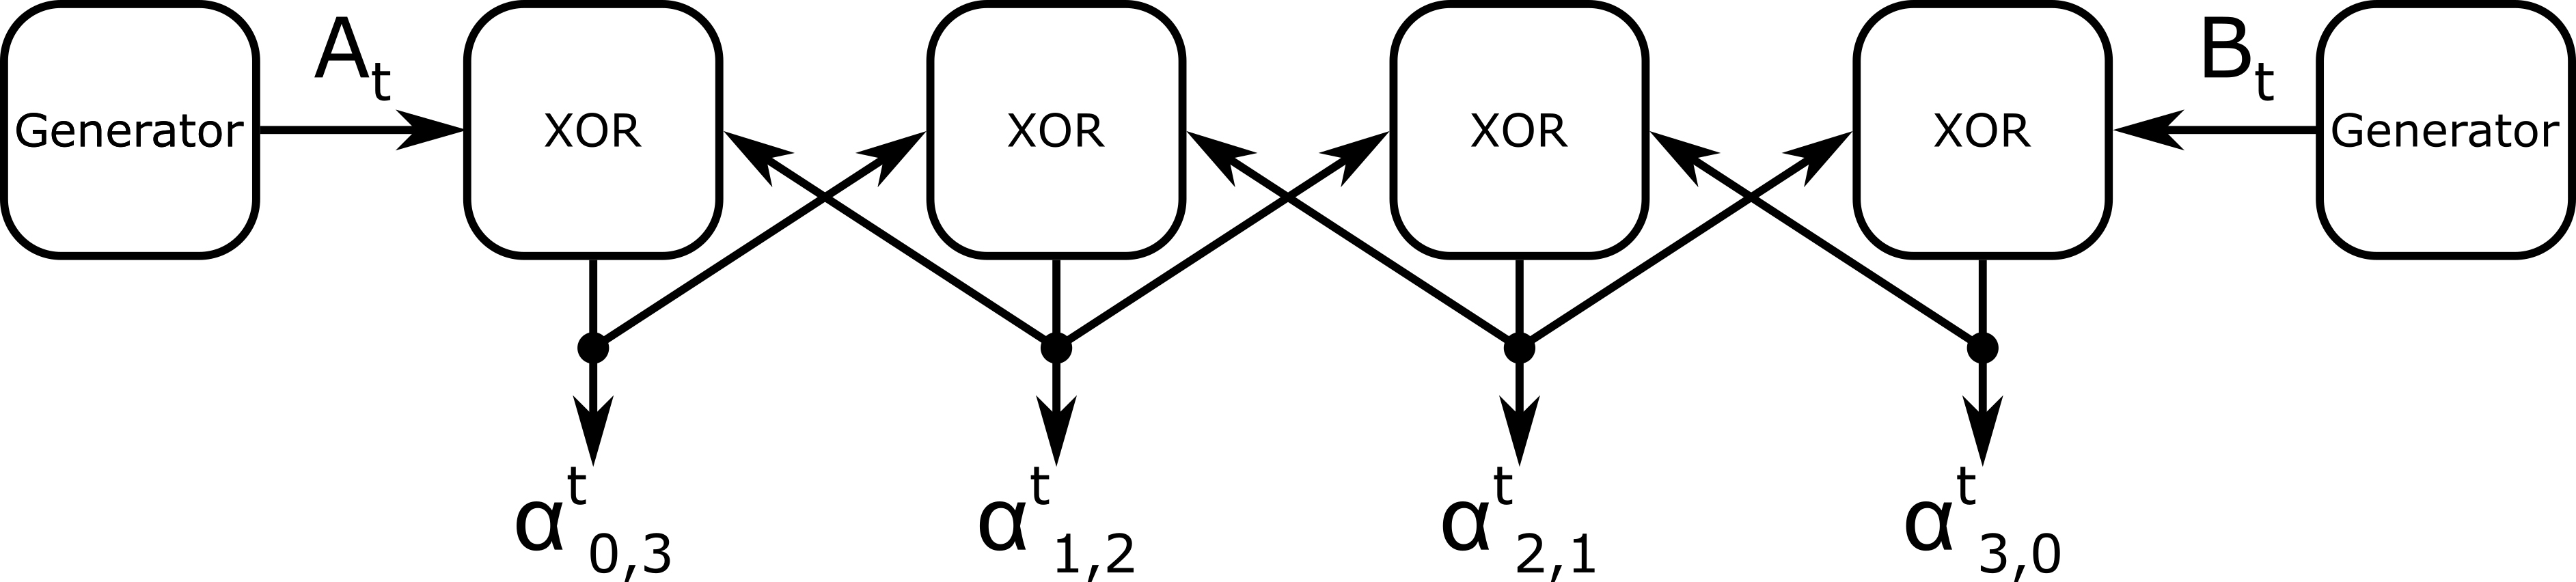
\includegraphics[width=\textwidth]{MISRN2.png}
\caption{Second scheme for producing MISRN by chaining exclusive-ors of }
\label{fig:scheme2}
\end{figure}

\begin{minipage}{1.0\textwidth}
\centering
\begin{lstlisting}[language=VHDL, caption={Scheme 2 implemented in VHDL. Although the functional code is shown spread over lines 7-8 here, the working code uses only one.} , label=lst:Scheme2]
ARCHITECTURE rtl OF XorChain2 IS
  SIGNAL Temp : tArray( -1 to N ) := (OTHERS=>(OTHERS=>'0'));
  SIGNAL Pipeline : tArray( 0 to N-1 ) := (OTHERS=>(OTHERS=>'0'));
BEGIN
  DataOut  <= Pipeline( 0 TO N-1 ); -- Mapping
  Temp     <= DataInA & Pipeline & DataInB; -- Mapping
  Pipeline <= Temp( -1 TO N-2 ) XOR Temp( 1 TO N )
                WHEN RISING_EDGE( Clk ); -- Clocked Logic
END ARCHITECTURE rtl;
\end{lstlisting}
\end{minipage}

You may reasonably question whether such a scheme results in terms ``cancelling out'', since $A \xor A = 0$.  



{\tiny
\begin{center}
\begin{tabular}{ c c c c c }
  Time, t & $\alpha^t_{(0,3)}                                    $ & $\alpha^t_{(1,2)}                  $ & $\alpha^t_{(2,1)}                  $ & $\alpha^t_{(3,0)}                          $  \\
 \hline
  0       & $                                               0$ & $                                               0$ & $                                               0$ & $                                               0$ \\  
  1       & $A_0                                             $ & $                                               0$ & $                                               0$ & $                                             B_0$ \\ 
  2       & $A_1                                             $ & $A_0                                             $ & $                                             B_0$ & $                                             B_1$ \\ 
  3       & $A_2 \xor A_0                                    $ & $A_1                                     \xor B_0$ & $A_0                                     \xor B_1$ & $                                    B_0 \xor B_2$ \\ 
  4       & $A_3 \xor A_1                            \xor B_0$ & $A_2                                     \xor B_1$ & $A_1                                     \xor B_2$ & $A_0                            \xor B_1 \xor B_3$ \\ 
  5       & $A_4 \xor A_2                            \xor B_1$ & $A_3                            \xor B_0 \xor B_2$ & $A_2 \xor A_0                            \xor B_3$ & $A_1                            \xor B_2 \xor B_4$ \\ 
  6       & $A_5 \xor A_3                   \xor B_0 \xor B_2$ & $A_4 \xor A_0                   \xor B_1 \xor B_3$ & $A_3 \xor A_1          \xor          B_0 \xor B_4$ & $A_2 \xor A_0                   \xor B_3 \xor B_5$ \\ 
  7       & $A_6 \xor A_4 \xor A_0          \xor B_1 \xor B_3$ & $A_5 \xor A_1                   \xor B_2 \xor B_4$ & $A_4 \xor A_2          \xor          B_1 \xor B_5$ & $A_3 \xor A_1 \xor          B_0 \xor B_4 \xor B_6$ \\
  8       & $A_7 \xor A_5 \xor A_1          \xor B_2 \xor B_4$ & $A_6 \xor A_2 \xor A_0          \xor B_3 \xor B_5$ & $A_5 \xor A_3          \xor B_0 \xor B_2 \xor B_6$ & $A_4 \xor A_2 \xor          B_1 \xor B_5 \xor B_7$ \\
  9       & $A_8 \xor A_6 \xor A_2 \xor A_0 \xor B_3 \xor B_5$ & $A_7 \xor A_3 \xor A_1 \xor B_0 \xor B_4 \xor B_6$ & $A_6 \xor A_4 \xor A_0 \xor B_1 \xor B_3 \xor B_7$ & $A_5 \xor A_3 \xor B_0 \xor B_2 \xor B_6 \xor B_8$ \\
  \vdots  & \vdots                                                 & \vdots                               & \vdots                               & \vdots                                        \\
\end{tabular}
\captionof{table}{Table showing the first few terms of MISRN scheme 2 for the case of a chain-length of four.}\label{tab:MISRN2a}
\end{center}
}

{\tiny
\begin{center}
\begin{tabular}{ c c c c c }
  Time, t & $\alpha^t_{(0,2)}$         & $\alpha^t_{(1,1)}$      & $\alpha^t_{(2,0)}$ \\
 \hline
  0       & $                    0$ & $           0$ & $                    0$ \\  
  1       & $A_0                  $ & $           0$ & $                  B_0$ \\ 
  2       & $A_1                  $ & $A_0 \xor B_0$ & $                  B_1$ \\ 
  3       & $A_2 \xor A_0 \xor B_0$ & $A_1 \xor B_1$ & $A_0 \xor B_0 \xor B_2$ \\ 
  4       & $A_3 \xor A_1 \xor B_1$ & $A_2 \xor B_2$ & $A_1 \xor B_1 \xor B_3$ \\ 
  \vdots  & \vdots                  & \vdots         & \vdots                  \\
\end{tabular}
\captionof{table}{Table showing the first few terms of MISRN scheme 2 for the special case of a chain-length of three.}\label{tab:MISRN2b}
\end{center}
}


\end{document}